\section{Variational-Based Mixed Noise Removal With CNN Deep Learning Regularization}

\begin{center}
    \author{
    Faqiang Wang,
    Haiyang Huang,
    Jun Liu
    }
\end{center}

\begin{center}
    \emph{IEEE TRANSACTIONS ON IMAGE PROCESSING, VOL.29, 2020}
\end{center}

\subsection{INTRODUCTION}
Random noise distributions correspond to standard probabilistic distributions, 
such as the Gaussian, Poisson and other distributions. There have 
been many methods that attempt to clean up noisy images. The classical 
methods are based on the use of filters such as Gaussian, Gabor or median 
filters. Other tools such as the Variational method have been widely used. 
This method is based on reducing the cost function containing the fidelity 
term of the data, useful for calculating the difference between true and observed 
data, and the regularization terms. Another method used was that of 
TV regularization. Unfortunately this method fails to preserve texture detail. 
Nonlocal methods, on the other hand, are able to capture image details. 
These methods exploit the self-similarity properties that can be integrated 
into variational methods. Despite these methods, the function of the weights 
is difficult to determine. Methods based on deep learning have achieved good 
noise reduction performance. Many of these assume that the value can be 
removed by applying the L2 norm. According to the study carried out in 
the following article, in order to remove the mixed noise it is necessary to 
determine the type and level of noise in each pixel. The methods based on 
the variation, unlike the neural networks, require a single image and can 
integrate different techniques of regularization useful to be able to remove 
the single noise and the mixed noise. The complexity of these methods lies 
in being able to create a non-computationally complicated design. In the 
proposed article, the EM (Expectation-Maximization) algorithm is used to 
remove the noise, with the integration of a CNN process as regularization, 
in order to create a new variational method. The method is able to iteratively 
estimate the noise parameters useful for classifying the type and level 
of noise in each pixel. The work carried out is divided into four phases: 
regularization, synthesis, parameter estimation and error classification.

\subsection{RELATED WORK}
\subsubsection{Mixed Noise Model}
The mixed noise is:
\begin{equation}
    n = \left\{ \\
    \begin{array}{cc}
        n_1, & with~probability~r_1,\\
        n_2, & with~probability~r_2,\\
        \cdots, & \cdots\\
        n_k, & with~probability~r_k,\\ 
    \end{array}
     \right\}
\end{equation}
where $ n_k $ is the \emph{k}-th noise component with probability density function (PDF) 
$ p_k $ and $ r_k $ are the unknown mixture ratios and thei sum is equal to 1.

\subsubsection{Weighted K-SVD Model}
The following work is based on the method proposed in \cite{0884882814}. After obtaining 
the value of the mixed-noise \emph{Probability Density Function} (PDF), and 
assuming that the noise has a uniform distribution, we can derive the \emph{negative 
log-likelihood} function (\ref{PDF}) useful as {\bfseries{fidelity term}} in the variational 
method. 
\begin{equation}\label{PDF}
    \mathcal{L}(u,\Theta) = - \sum_{x\in\Omega}\ln\sum_{k=1}^Kr_kp_k(u(x)-f(x))
\end{equation}
In order for this probability to be extended to more types of noise 
distribution, it is necessary to perform an optimization that minimizes the 
upper limit of the function (\ref{H function}). 
\begin{eqnarray}\label{H function}
    \mathcal{H}(u,\Theta,w) & = & - \sum_{x\in\Omega}\sum_{k=1}\ln\left[r_kp_k(u(x)-f(x))\right]w_k \nonumber \\
                  &   & + \sum_{x\in\Omega}\sum_{k=1}w_k(x)\ln{w_k(x)}  
\end{eqnarray}
To minimize $\mathcal{H}$, a minimization of $ w $ must be performed, which is a probability 
indicates the noise at each pixel, and an iterative minimization of the other 
two variables $ u $ and $ \Theta $.

\subsubsection{IRCNN}
Another method \cite{0884882819} uses a CCN, based on the IRCNN model, to restore an 
image in which Gaussian noise is present. In this model, patches based $ L^2 $ 
residual loss functions are adopted. Unfortunately, if there are mixed-noises, 
this method does not produce satisfactory results.

\subsection{THE PROPOSED METHOD (EM-CNN)}
In the following paper a general variational model is proposed, formed by 
the combination of a deep learning method and variational methods, with 
regularized CNN to remove the mixed-noise problem, especially noises such 
as the Gaussian mixture and the Gaussian-impulse.

\subsubsection{General Model}
Removal of mixed-noise can be done with the following model:
\begin{equation}\label{HFunction}
    (u^*, \Theta^*, w^*) = \argmin_x\left\{H(u,\Theta,w) + \lambda_1\mathcal{J}(u)\right\}
\end{equation}
where $\mathcal{J}$ is a regularizer, such \emph{Total Variation Regularization} (TV) while $ \lambda_1 $ 
control the balance of the terms. By changing $u$ with an auxiliary function 
$v$, and applying the \emph{augmented Lagrangian method} (ALM) \cite{0884882833}, the minimizations 
on each component of $\mathcal{H}$ ($u$, $\Theta$, $w$) change. The resolution of these 
minimizations allows to divide the mixed-noise removal problem into Gaussian 
noise removal (renewing $u$), choice of the fidelity term (renewing $v$), 
noise reduction (updating the Lagragian multiplier $u$), parameter estimation 
noise ($\Theta$ update) and error classification ($w$ update). The formula used by 
the model is able to handle different types of Gaussian noises such as impulse 
noise, mixed-noise Gaussian-impulse and many others. Each noise has 
a certain probability function pk, so just change this value in (\ref{H function}). A CNN 
can be used to learn Gaussian noise for different types of levels. In this paper 
the CNN based denoiser \cite{0884882819} was used. The weight $w$ is useful for assigning 
different fidelity terms to pixels contaminated by different levels of types of 
noise. The minimization of $\Theta$ and $w$ are part of EM processes. Thanks to 
these it is possible to extract information such as noise variations and the 
classification of this in different classes. In summary, the minimizations to 
be calculated are the following:

\begin{equation}\label{uMin}
    u^{v+1} = \argmin_u \lambda_1\mathcal{J}(u)+\mathcal{H}(u,\Theta^v,w^v),
\end{equation}
\begin{equation}\label{ThetaMin}
    \Theta^{v+1} = \argmin_\Theta \mathcal{H}(u^{v+1}, \Theta, w^v),
\end{equation}
\begin{equation}\label{wMin}
    w^{v+1} = \argmin_{w\in{S}} \mathcal{H}(u^{v+1}, \Theta^{v+1},w)
\end{equation}

\subsubsection{Gaussian Mixture Model}
A Gaussian mixture model is a probabilistic model that assumes all the data 
points are generated from a mixture og finite number of Gaussian distributions 
with unknown parameters. The distributions of Gaussian noises change 
according to the assumed variance ($\sigma^2$) value. The new function $ \mathcal{H} $ will be 
as follows:
\begin{eqnarray}\label{HFunctionGMM}
    \mathcal{H}(u,r,\sigma^2,w) & = & \frac{1}{2}\sum_{x\in\Omega}\sum_{k=1}^K\frac{(u(x)-f(x))^2}{\sigma^2_k}w_k(x)-\sum_{x\in\Omega}\sum_{k=1}^Kw_k(x)\ln{r_k}\nonumber \\
                                &   & + \frac{1}{2}\sum_{x\in\Omega}\sum_{k=1}^Kw_k(x)\ln{\sigma^2_k}+\frac{1}{2}\sum_{x\in\Omega}\sum_{k=1}^Kw_k(x)\ln{w_k}(x)
\end{eqnarray}
The optimizations (\ref{uMin}) (\ref{ThetaMin}) (\ref{wMin}) of the parameters of (\ref{HFunctionGMM}) are adapted by 
including the two new parameters $r$ and $\sigma^2$, enclosed in $\Theta$, which will be minimized 
in turn. Through the optimization of these parameters it is possible to remove 
the mixed-noise Gaussian. In summary, all the steps carried out are 
illustrated in figure \ref{fig:EM-CNN}.
\begin{figure}[h!]
    \centering
    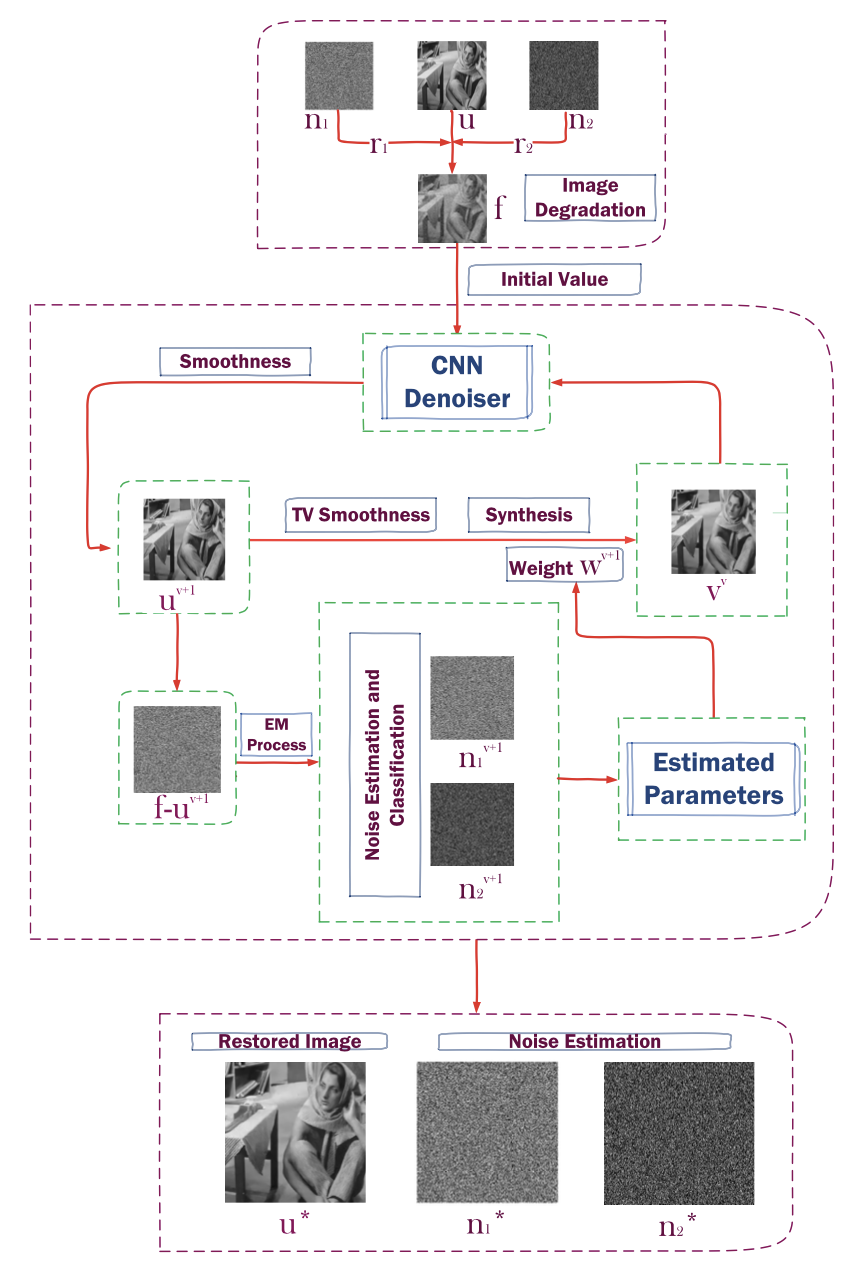
\includegraphics[width = 0.7 \linewidth]{images/paper7/flowchart.png}
    \centering
    \caption{The flowchart of EM-CNN algorithm.}
    \label{fig:EM-CNN}
\end{figure}
Image degradation occurs using the additive noise model: 
$$ f = u + n $$
where $f$ is the observed image (the one resulting from the combination of 
noises), $u$ is the true image and $n$ is the introduced noise. The image $f$ will 
be the input of the CNN network which, through its denoise \cite{0884882819}, will perform 
a smoothing on the image obtaining a new image $u^{v+1}$. CNN applies two 
operations on this image in parallel. The first is that of the noise put back 
in which the noise present in the image f is extracted by simply subtracting 
the image $u^{v+1}$. Subsequently, to calcutale the fidelity term, the EM algorithm 
\cite{0884882814} is applied to this noise which has the task of estimating the error 
and classifying it by minimizing the terms of \ref{HFunctionGMM}. The minimization of each 
weight $w$ leads to a continuous updating of this parameter which translates 
into greater precision in determining the noise on each individual pixel. The 
estimation of the parameters allows to carry out the synthesis process, or to 
select a new fidelity term, for each pixel, based on the estimates made on the 
noise. The second operation is to apply the \emph{Total Variation Regularization} 
(TV) \cite{0884882802} on the starting image $u^{v+1}$ useful for carrying out a good 
restructuring of the image from noise and blurred data. The image $V^v$ with the 
updated w weights, will be the new input of the CNN network that through 
multiple iterative processes will improve until its convergence, or until the 
fidelity term will no longer change. The output returned by the model will 
consist of a restructured image ($u^*$) accompanied by the estimates of the 
individual noises ($n_1^ *, n_2^*$) applied at the beginning.

\subsubsection{Gaussian Noise Plus Impulse Noise}
The overall noise can consist of several noise distributions. Previously, the 
operations useful for obtaining information on a Gaussian noise distribution 
have been defined. When the Gaussian distribution assumes random values 
(called salt and pepper), and therefore not uniformly distributed, then the 
optimization problem becomes more difficult. In order to find a solution, it 
is necessary to approximate a part of the PDF concerning the random-value 
noise by a Gaussian function, which means that it is possible to use the 
Gaussian mixture noise model to optimize the Gaussian plus impulse noise.

\subsection{EXPERIMENTAL RESULTS}
The experiments are conducted on mixed-noise Gaussian noise and on Gaussian 
plus impulse noise. The indices used to estimate the quality of the restructured
images are the \emph{Signal-to-Noise Ratio} (PSNR) and the \emph{Structural 
Similarity Index} (SSIM) \cite{0884882841}.

\subsubsection{Gaussian Mixed Noise}
The quality comparison is done with different methods already existing in 
the state of the art. From figure \ref{fig:GMNComp} you can see the application of 
each of these methods on an image in which there is the presence of mixed-noise. 
The proposed method produces a restructured image with a better level of 
texture detail.
\begin{figure}[h!]
    \centering
    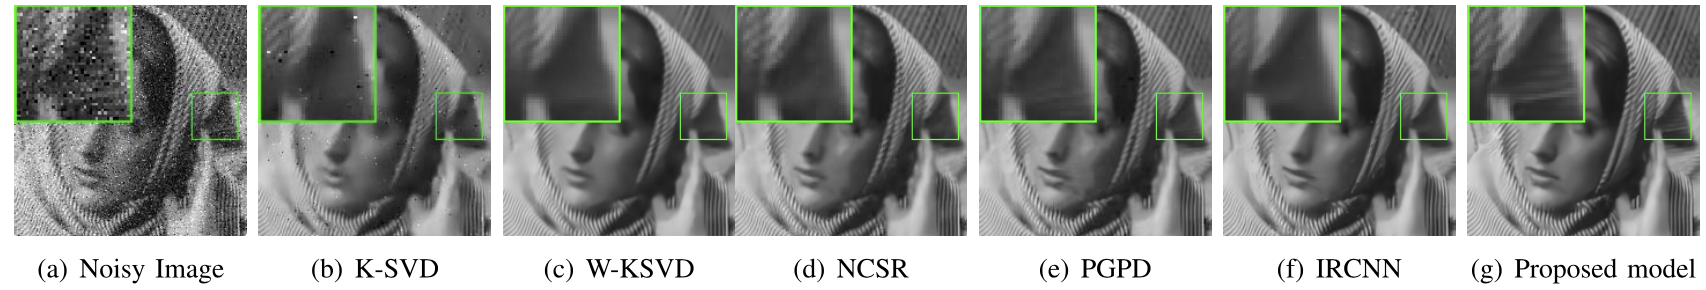
\includegraphics[width = \linewidth]{images/paper7/GMN comparison.png}
    \centering
    \caption{Image reconstruction under Gaussain mixture noise comparison.}
    \label{fig:GMNComp}
\end{figure}

To test the efficiency of the methods, several images belonging to a 
BSD100 dataset \cite{0884882842} were taken on which there are two Gaussian noises ($n_1$ 
and $n_2$) with different mixture $r_1, r_2$ and standard deviation ($\sigma$). By comparing the 
results obtained in table \ref{indexCompare}, the proposed method achieves the highest values 
in both indices compared to the two methods \cite{0884882815} \cite{0884882819} most common in the 
state of the art.
\begin{table}[h!]
    \centering
    \begin{adjustbox}{max width=\textwidth}
    \begin{tabular}{|c||ccc|ccc|ccc|}
        \hline
            & \multicolumn{3}{c||}{$\sigma_1=5 ~~~\sigma_2=30 $} & \multicolumn{3}{c||}{$\sigma_1=10 ~~~\sigma_2=50 $} & \multicolumn{3}{c||}{$\sigma_1=15 ~~~\sigma_2=75 $}\\
        \hline        
        $r_1:r_2\rightarrow$ & 0.3:0.7 & 0.5:0.5 & 0.7:0.3 & 0.3:0.7 & 0.5:0.5 & 0.7:0.3 & 0.3:0.7 & 0.5:0.5 & 0.7:0.3\\
        \hline 
        \hline
        \multirow{2}{*}{PGPD\cite{0884882815}} & 29.42 & 30.16 & 31.19 & 27.23 & 27.88 & 28.78 &25.64 & 26.26 & 27.14\\
        & 0.8132 & 0.8349 & 0.8544 & 0.7404 & 0.7634 & 0.7874 & 0.6790 & 0.7044 & 0.7336\\
        \hline
        \multirow{2}{*}{IRCNN\cite{0884882819}} & 29.83 & 30.53 & 31.48 & 27.66 & 28.25 & 29.04 & 19.37 & 25.22 & 27.32\\
        & 0.8262 & 0.8451 & 0.8664 & 0.7611 & 0.7789 & 0.7993 & 0.2948 & 0.6423 & 0.7426\\
        \hline
        \multirow{2}{*}{Proposed} & \bfseries{29.88} & \bfseries{31.26} & \bfseries{32.72} & \bfseries{28.01} & \bfseries{29.00} & \bfseries{30.37} & \bfseries{26.23} & \bfseries{27.41} & \bfseries{28.84}\\
        & \bfseries{0.8273} & \bfseries{0.8785} & \bfseries{0.9094} & \bfseries{0.7801} & \bfseries{0.8112} & \bfseries{0.8528} & \bfseries{0.6931} & \bfseries{0.7613} & \bfseries{0.8077}\\
        \hline
    \end{tabular}
    \end{adjustbox}
    \caption{Average PSNR and SSIM values on BSD100 datasets of some methods.}
    \label{indexCompare}
\end{table}
